\section{Tratamientos de datos multidimensionales}

\subsection{Compresión y \textit{denoising} de señales bidimensionales}
Uno de los grandes problemas ligados al manejo de datos multidimensionales es su tamaño en memoria. En experimentos que requieran el trabajo simultáneo de todos los sensores, la cantidad de bytes necesaria para guardar la información de una única muestra puede llegar al orden de varios gigabytes. Por ello se hace tan tedioso trabajar con este tipo de datos, y necesitamos métodos de compresión que nos ayuden en nuestras tareas de análisis. También hablaremos de \textit{denoising} (filtrado del ruido) porque estos mismos algoritmos van a dar muy buenos resultados.

\subsubsection{\textit{Fast Fourier transform} (FFT)}
Atendiendo a la definición de la transformada de Fourier, toda función periódica puede ser descrita como una base ortogonal de senos o cosenos. Si nos vamos al caso discreto, dada una sucesión de $n$ puntos tendremos:

\begin{equation}
     \hat f_k = \sum^{n-1}_{j=0} f_j e^{-i2\pi j k/n}
     \qquad\qquad
     f_k = \frac{1}{n} \left( \sum^{n-1}_{j=0} \hat f_j e^{-i2\pi j k/n} \right)
\end{equation}\\

El algoritmo FFT nos permite calcular los coeficientes $f_j$ con un ínfimo coste computacional. De este modo, podremos codificar en el espacio recíproco gran cantidad de información en cuestión de milisegundos.\\

La clave de trasladar nuestra imagen al espacio recíproco está en imponer un umbral al valor absoluto de los coeficientes $f_j$. Así somos capaces de seleccionar las frecuencias más significativas, que serán las que almacenemos en memoria como una matriz de números complejos tipo \textit{float} de 4 bytes y valores lógicos de 1 bit para aquellas componentes nulas. De este modo lograremos reducir considerablemente el espacio en memoria ocupado por la información de nuestra imagen. Una vez que queramos reconstruir la imagen comprimida no tendremos más que cargar dicha matriz y aplicar la FFT inversa.\\

Para cuantificar esta compresión, se define el coeficiente de ratio de compresión $CR$ como una relación proporcional entre el tamaño de la imagen original $S_o$ y el de la imagen ya comprimida $S_c$:

\begin{equation} \label{cr}
   S_c = CR \cdot S_o 
\end{equation}

En el caso de la \autoref{fig:3}, tenemos una imagen original con profundidad de 2 bytes (\textit{uint16}). Al aplicar el algoritmo explicado previamente y calcular el ratio de compresión, observamos una reducción en el tamaño de más de cinco veces respecto al tamaño original. Estos resultados son bastante impresionantes, más aún si tenemos en cuenta que además de aplicar una compresión logramos reducir el ruido de forma considerable, pues estamos capturando la periodicidad de la red (ver el caso \ref{fig:3}a).

\begin{figure}[h!]
    \centering
    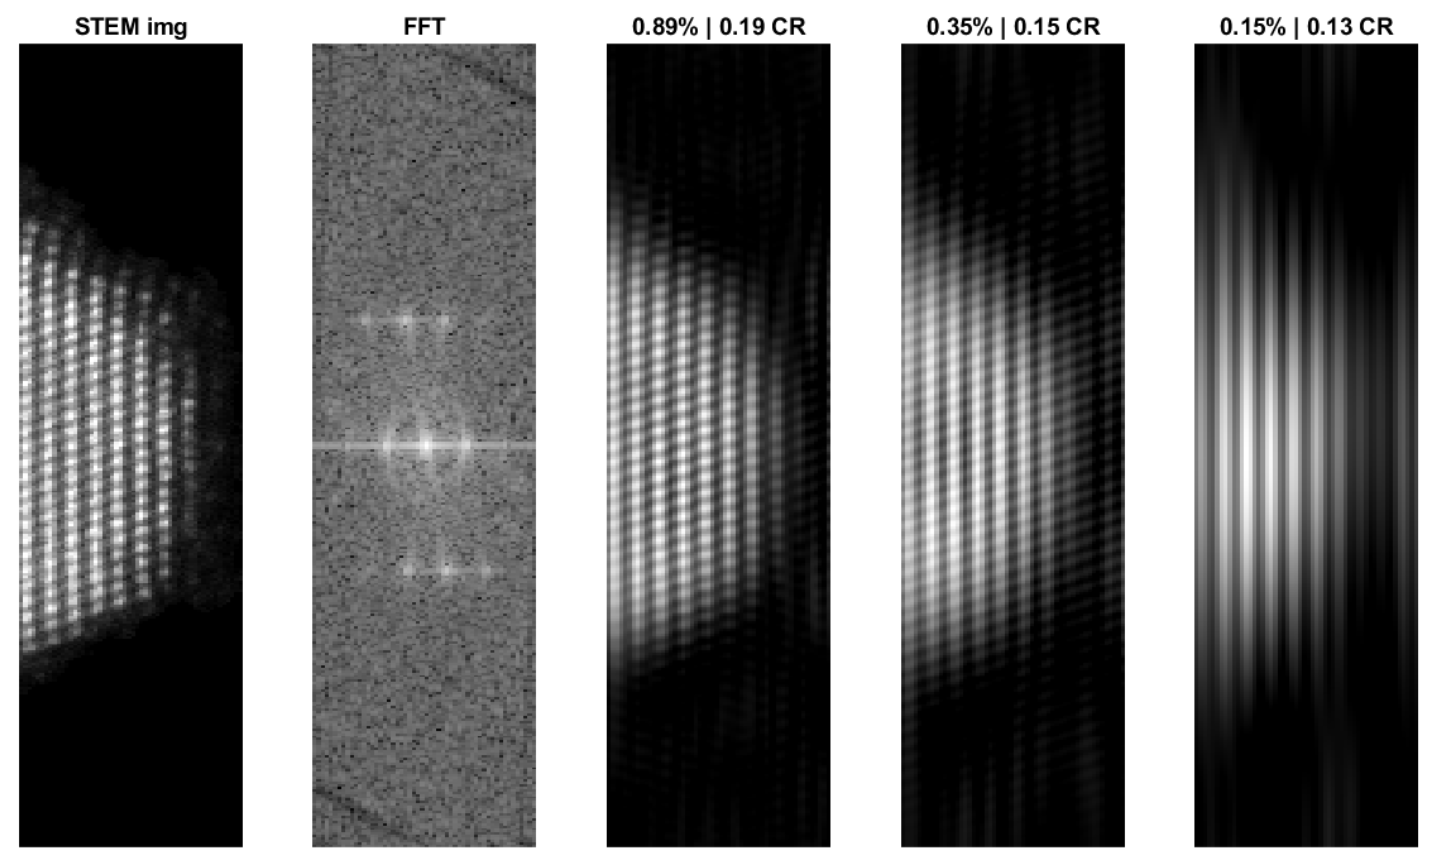
\includegraphics[width=1\textwidth]{fig/Fig3.png}
    \caption{Dada una imagen STEM ADF de tungsteno (111) \cite{datos}, tomamos la FFT para visualizar su información en el espacio recíproco. Posteriormente se aplican una serie de umbrales que eliminan los coeficientes menos significativos de la transformada, para cada caso se indica en el título el porcentaje de coeficientes no nulos respecto al total y el ratio de compresión. El código ha sido desarrollado en MATLAB por el autor y se puede encontrar en \cite{repo}. }
    \label{fig:3}
\end{figure}

Aunque únicamente hemos puesto como ejemplo una imagen ADF, este método de compresión y limpiado de ruido funciona de forma similar para BF, patrones de difracción en el espacio recíproco e imágenes que representen una integración de todos los canales de energía en cada punto (EELS \textit{mean image}).

\subsubsection{\textit{Singular value decomposition} (SVD)}

Dada una matriz $A$ con dimensiones $m \times n$, sus valores singulares corresponderán con la raíz cuadrada de los autovalores de $A^T A$, que vendrán denotados por $\sigma_1$, $\dots$, $\sigma_n$ y ordenados de forma que $\sigma_1 \geq \sigma_2 \geq \dots \geq \sigma_n$. Con esto en mente, se puede demostrar \cite{biblia} que existe una descomposición tal que $A = U \Sigma V^T$, donde U ($m \times m$) y V ($n \times n$) son matrices ortogonales y $\Sigma$ ($m \times n$) es una matriz diagonal compuesta por $\sigma_1$, $\dots$, $\sigma_n$. \\

Interpretaremos A como una transformación que nos lleva del dominio $\mathds{R}^n$ hasta el rango $\mathds{R}^m$. Como es de esperar, ambos espacios podrán ser descritos por una base vectorial, que vendrá contenida en las matrices V (dominio) y U (rango). Con esto en mente, ya somos capaces de visualizar la SVD como una método que se asegura de encontrar un par de bases ortonormales tales que la transformación quede representada por la matriz diagonal $\Sigma$. \\

\newpage
\begin{figure}[h!]
    \centering
    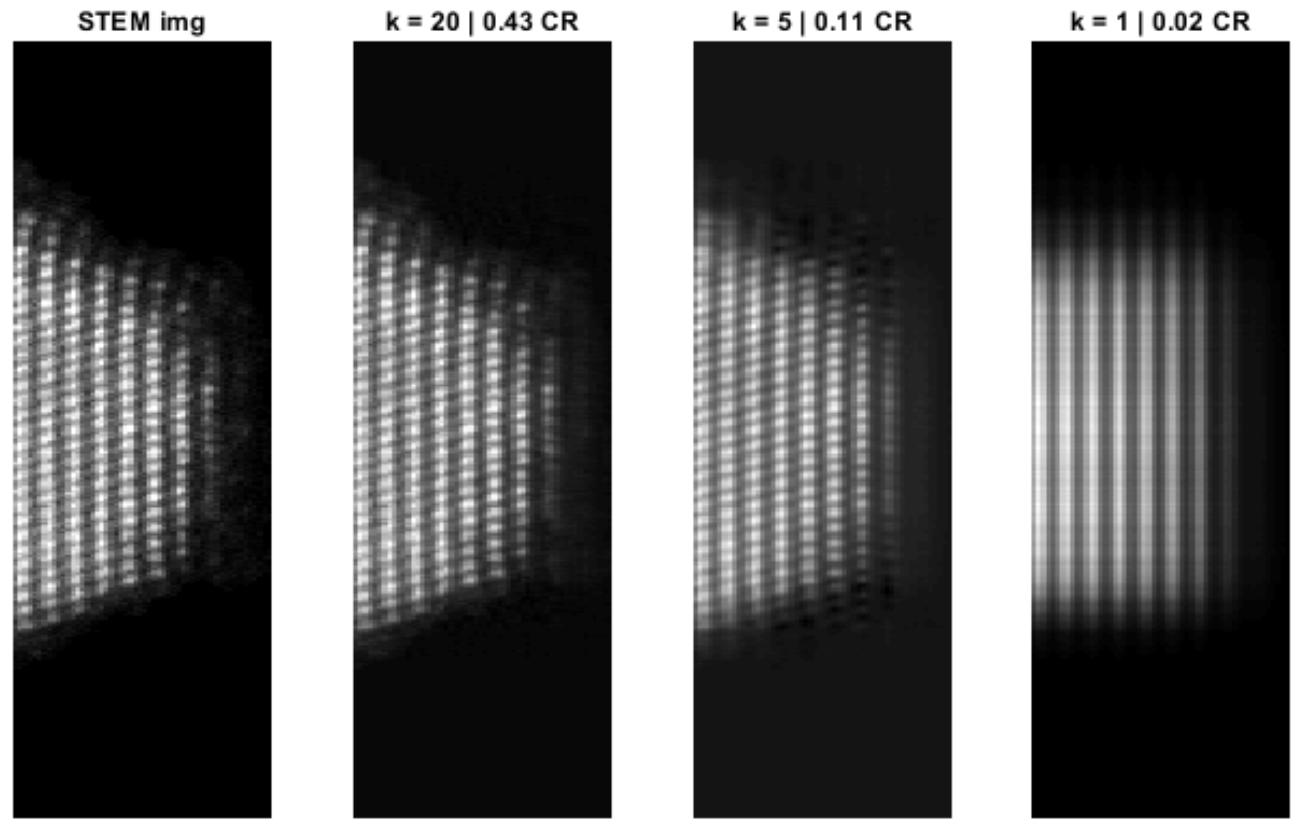
\includegraphics[width=0.85\textwidth]{fig/Fig4.png}
    \caption{Sobre la misma imagen STEM de la \autoref{fig:3} se ha realizado una descomposición SVD. En la figura se muestra la imagen que resulta de tomar los  $k$ valores singulares indicados, junto al ratio de compresión. Programa desarrollado en MATLAB por el autor \cite{repo}.}
    \label{fig:4}
\end{figure}

\vspace{-0.2cm}
Para construir la matriz $V = [v_1 \dots v_n]$, se debe encontrar una base ortonormal $\{v_1, \dots, v_n\}$ compuesta por autovectores de la matriz simétrica $A^T A$. Estos mismos elementos $v_i$ se aprovechan para diseñar la matriz $U = [u_1 \dots u_m]$ tomando los vectores $Av_1, \dots, Av_n$, que también serán ortogonales (demostración sencilla en \cite{biblia}). \\

Bajo esta construcción, resulta que $||A v_i|| = A^T A$, de modo que cada elemento $A v_i$ se asocia a un valor singular de A. El problema de esto es que únicamente existen $r < m$ $\sigma_r \neq 0$, por lo que inicialmente no contaremos con la cantidad suficiente de vectores $A v_i$ para formar una base de $\mathds{R}^m$, tendremos que prolongar el conjunto $\{u_1 \dots u_r\}$ de dichos vectores normalizados. Teniendo todo esto en mente, finalmente obtendremos la base $\{u_1 \dots u_m\}$, donde $u_i = \frac{A v_i}{||A v_i||} = \frac{A v_i}{\sigma_i}$. \\

Una vez llegados a este punto, ya somos capaces de
desarrollar $A = U \Sigma V^T$ para llegar a una de las propiedades fundamentales de esta descomposición (\textit{low rank approximation property}): 

\begin{equation*}
    \begin{array}{ll}
        A = U 
        \begin{bmatrix}
        \sigma_1 & \cdots & 0        \\
        \vdots   & \ddots & \vdots   \\
        0        & \cdots & \sigma_r \\
        \end{bmatrix}
        V^T & = U
        \left(
        \begin{bmatrix}
        \sigma_1 & \cdots & 0        \\
        \vdots   & \ddots & \vdots   \\
        0        & \cdots & 0        \\
        \end{bmatrix} + \cdots +
        \begin{bmatrix}
        0        & \cdots & 0        \\
        \vdots   & \ddots & \vdots   \\
        0        & \cdots & \sigma_r \\
        \end{bmatrix}
        \right) V^T\\
        \\
         & = \sigma_1 u_1 v_1^T + \cdots + \sigma_r u_r  v_r^T,
    \end{array}
\end{equation*}

es decir, dada una matriz $A$ con dimensiones $m \times n$ y rango $r$ siempre se cumplirá

\begin{equation} \label{eq:SVD}
    A = \sum^r_{i=1} \sigma_i u_i v_i^T 
\end{equation}

Aprovechando esta propiedad podremos obtener una $A_{ap}$ similar a la matriz $A$, mediante una aproximación en mínimos cuadrados que coincidirá con los $k$ primeros términos de la ecuación (\ref{eq:SVD}). Cabe destacar que el rango de $A_{ap}$ será dicho $k \leq r$. \\

\subsection{Detección de columnas atómicas}

Automatizar la detección de máximos y mínimos en nuestras imágenes es un paso fundamental. Necesitamos codificar las posiciones de las distintas columnas atómicas para posteriormente ser capaces de extraer la información relevante del sistema. Para ello recurriremos a distintas técnicas de visión por ordenador que nos permitan detectar picos de intensidad. 

\begin{figure}[h!]
    \centering
    \includegraphics[width=1\textwidth]{fig/Fig5.png}
    \caption{Imagen generada en MATLAB por el autor \cite{repo} que muestra el caso de un \textit{blob} unidimensionales sobre los que se convoluciona distintos filtros NLoG. En la primera columna tenemos un \textit{blob} estrecho que puede ser capturado por una gaussiana de bajo $\sigma$. En la segunda y tercera columna contamos con un \textit{blob} más largo que requiere de una gaussiana con mayor $\sigma$ para que la señal convolucionada cuente con un pico bien definido. Finalmente, la última columna muestra la convolución de una señal con dos \textit{blobs}.}
    \label{fig:5}
\end{figure}

Aunque existen numerosos métodos, nosotros nos centraremos en los \textit{scale-space methods} por ser los más usados en STEM. Tal y como se observa en la \autoref{fig:5}, estos algoritmos toman inicialmente una señal matemática (filtro) y la convolucionan con la imagen real. En este caso trataremos el filtro NLoG (\textit{normalized Laplacian of Gaussian}). No obstante, también suelen usarse la DoG (\textit{difference of Gaussians}), el HoG (Hessian of Gaussian) y la CHT (\textit{circle Hough Transform}, ver \autoref{fig:6}). La magia de aplicar estas funciones reside en la forma de la señal convolucionada, pues si tomamos su valor absoluto presentará máximos en aquellos puntos donde la intensidad de la señal imagen es mayor. Comúnmente, la forma de dicha convolución dependerá del escalado del filtro, que en el caso del NLoG podremos controlar con un parámetro que llamaremos $\sigma$, como se muestra en la \autoref{eq:NLoG}.\\

\begin{equation} \label{eq:NLoG}
    NLoG(x,y,\sigma) = \sigma^2\nabla^2 n_\sigma =  - \frac{1}{\pi\sigma^2}\left[1 - \frac{x^2 + y^2}{2\sigma^2}\right]e^{-\frac{x^2 + y^2}{2\sigma^2}}
\end{equation}\\

Estos máximos de la señal final no siempre se encontrarán bien definidos, dependerá del tamaño del pico de intensidad en la imagen y de la forma de la gaussiana. Es más, existe una relación proporcional entre $\sigma$ para el que aparece el máximo y el tamaño del punto brillante, que podremos aprovechar para filtrar el ruido y evitar la detección de falsas columnas atómicas.\\

Al aplicar esta señal con varios valores de $\sigma$ generamos un volumen de imágenes apiladas:

\begin{equation}
    S(x,y,\sigma) = \sigma^2\nabla^2 n_\sigma \cdot I(x,y)
\end{equation}\\

De este modo, dada una imagen $I(x,y)$, podremos encontrar el conjunto de puntos brillantes ($x^*$,$y^*$) de tamaño $\sigma^*$ sin más que buscar los máximos dentro de dicho volumen S:

\begin{equation}
    (x^*,y^*,\sigma^*) = \underset{(x,y,\sigma)}{\text{arg max}} \; |\sigma^2 \nabla^2 n_\sigma \cdot I(x,y)|
\end{equation}\\

\begin{figure}[h!]
    \centering
    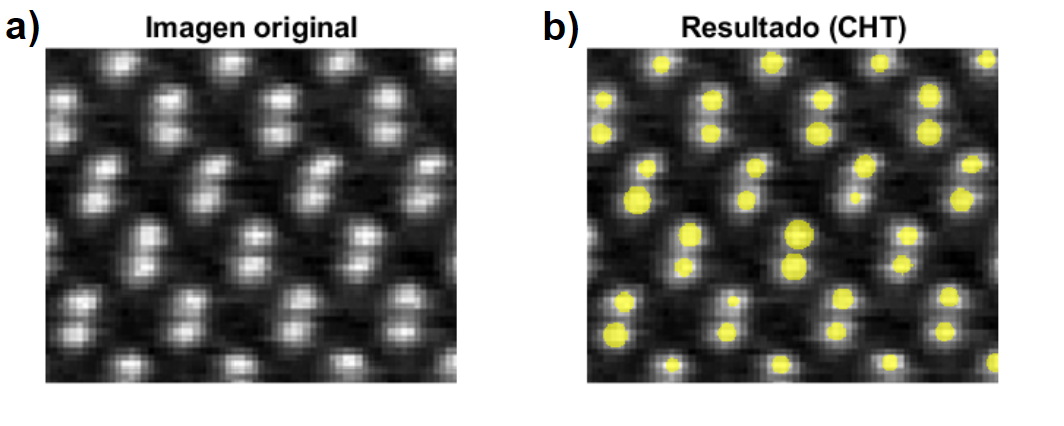
\includegraphics[width=0.9\textwidth]{fig/Fig6.png}
    \caption{Sobre una imagen ADF de GaAs \cite{maria} se utiliza la funcionalidad \textit{Circle Finder} de la aplicación \textit{Image Segmenter} incluida en el paquete \textit{Image Processing and Computer Vision} de MATLAB, que aplica la CHT \cite{matlab_circulos} como filtro para encontrar círculos de cierto radio.}
    \label{fig:6}
\end{figure}

\newpage
\begin{figure}[h!]
    \centering
    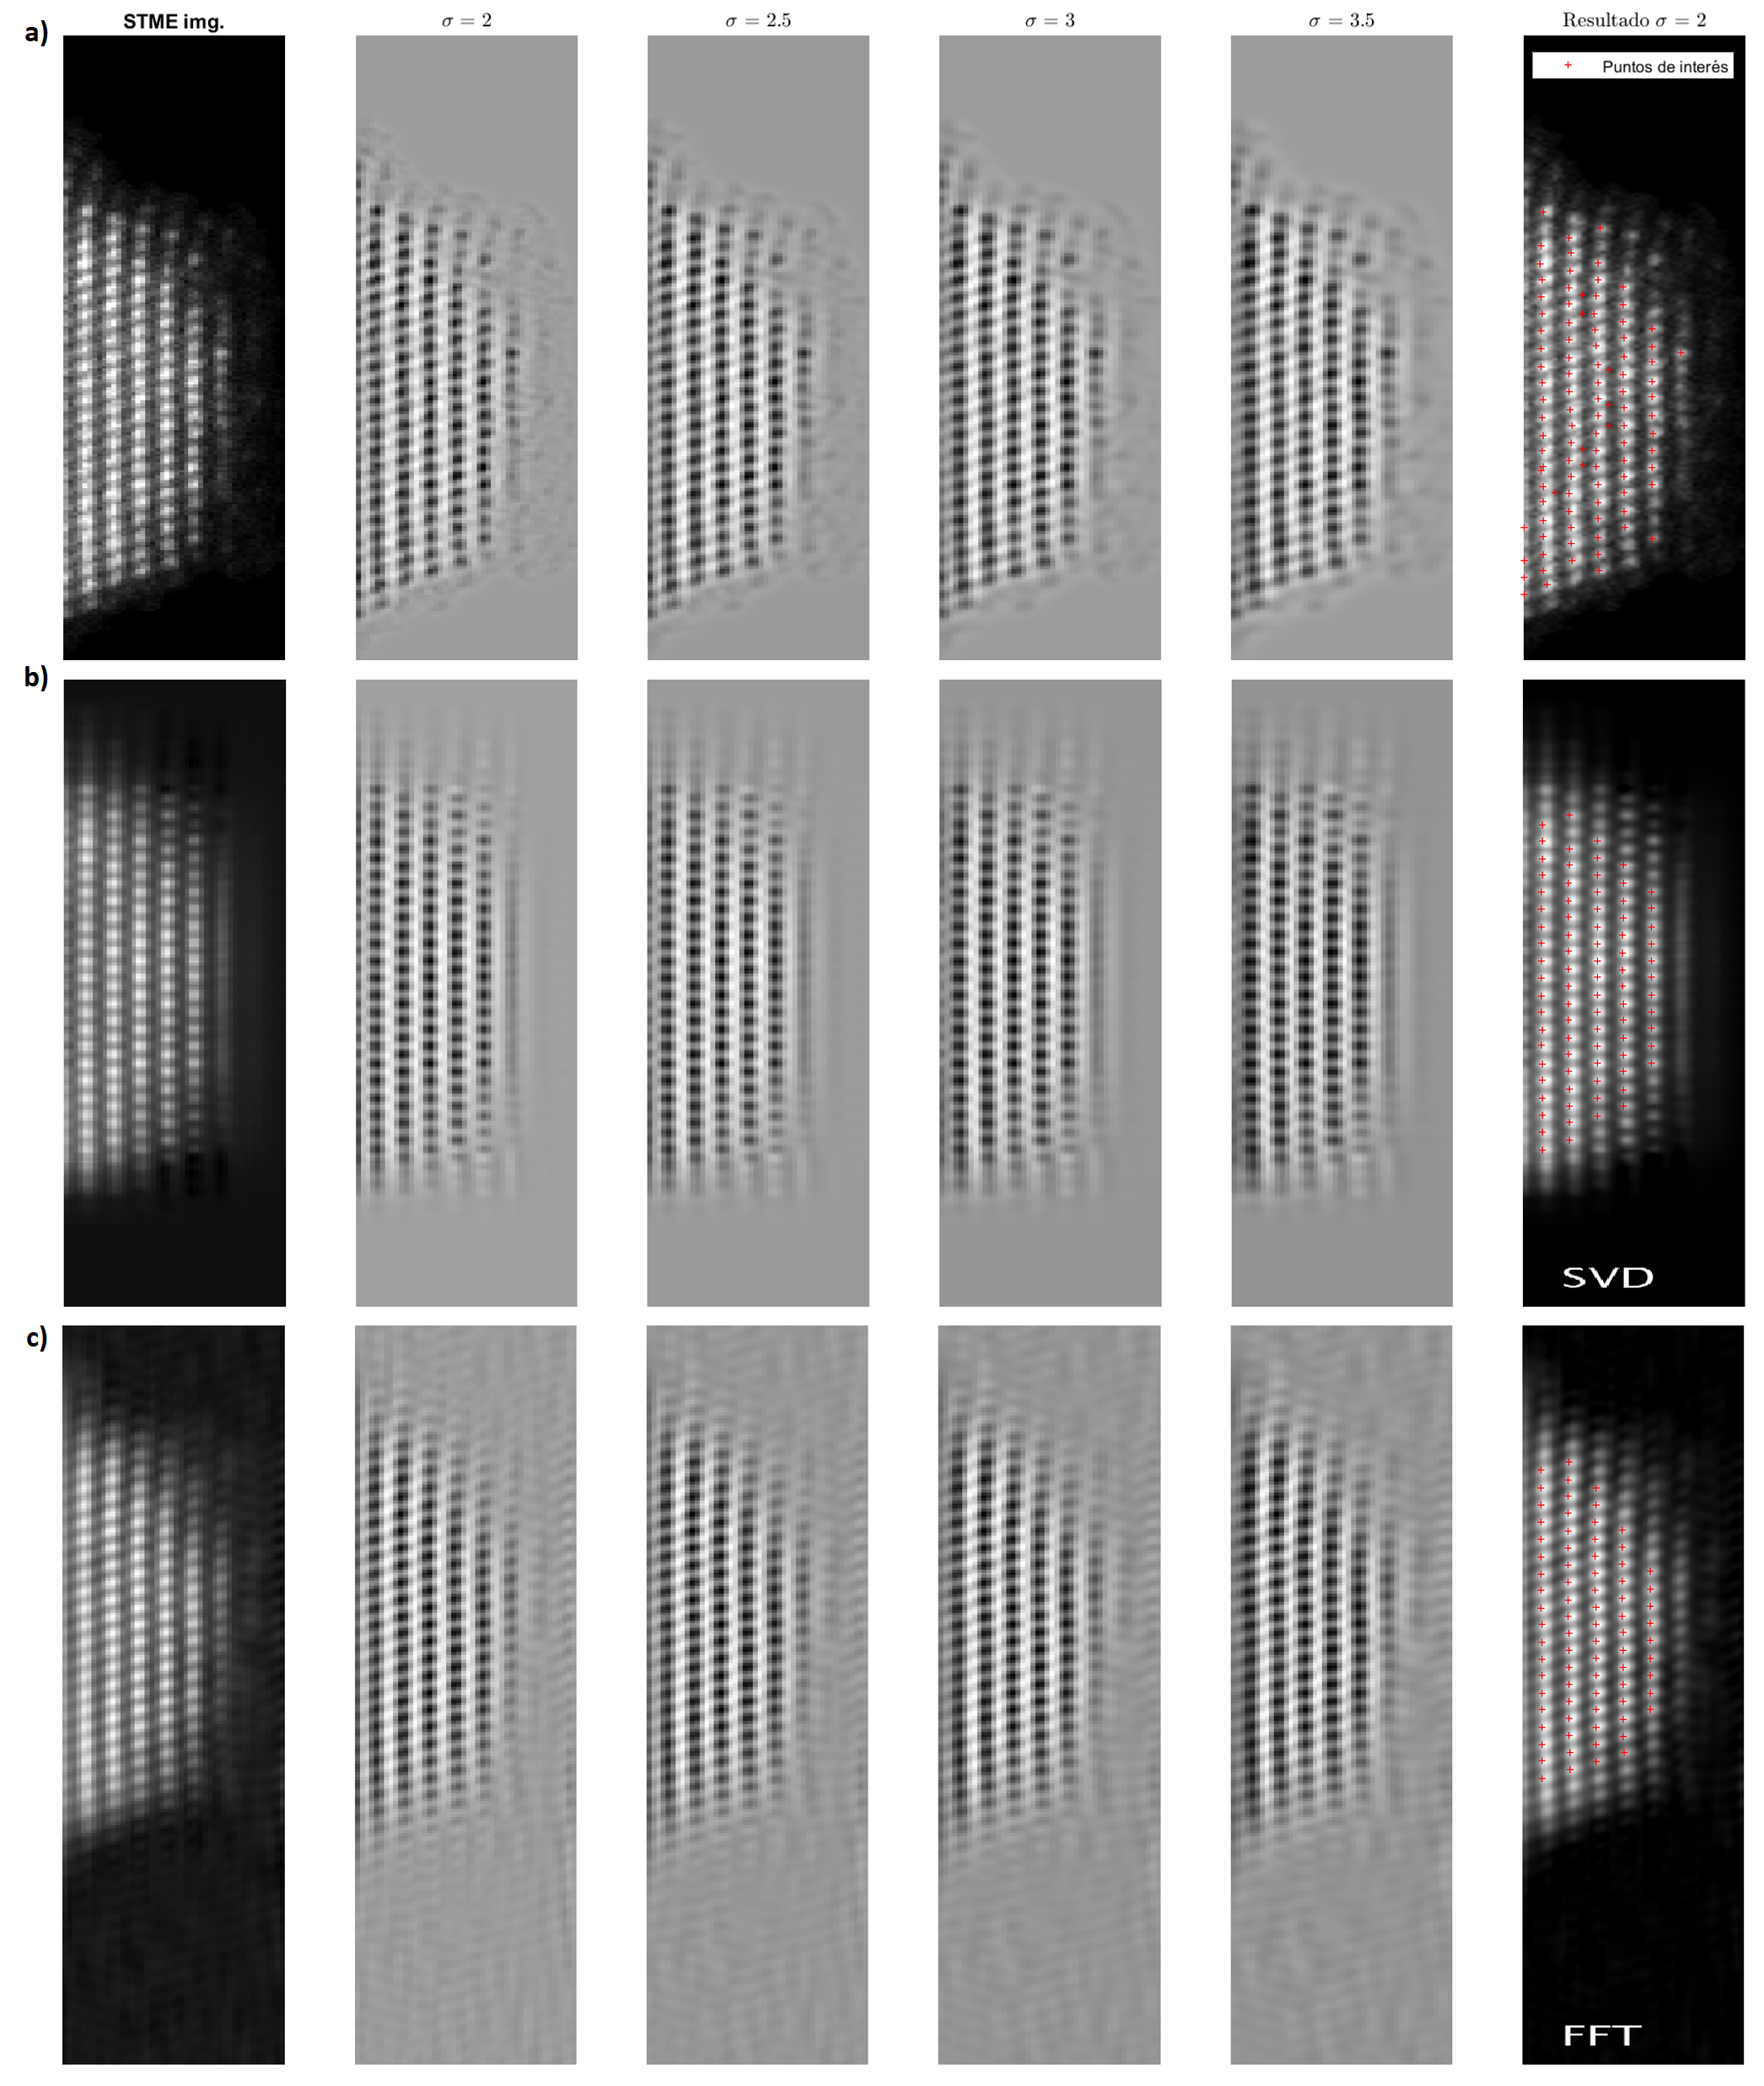
\includegraphics[width=1\textwidth]{fig/Fig7.png}
    \caption{Tomando la misma imagen ADF de la \autoref{fig:3}. En todos los casos se muestra la imagen de entrada junto a los planos del volumen $S$ que han sido generados aplicando el filtro NLoG para los valores indicados de $\sigma$. Una vez el algoritmo ha encontrado los blobs para $\sigma = 2$, se expone el resultado obtenido. En \textbf{a)} tenemos la imagen original, en \textbf{b)} y \textbf{c)} se ha aplicado SVD y FFT por separado para reducir el ruido. Programa desarrollado en MATLAB por el autor \cite{repo}.}
    \label{fig:7}
\end{figure}

\newpage

En la \autoref{fig:7} se muestra un ejemplo de este algoritmo programado en MATLAB por el autor. Como se puede observar, los resultados son satisfactorios siempre y cuando no nos encontremos cerca de la frontera de la red. También se aplica el algoritmo de detección a una imagen filtrada por SVD para mostrar que podemos obtener mejores resultados si tratamos la entrada reduciendo el ruido y saturando  los puntos brillantes.


